\documentclass[10pt,a4paper,catalan]{article}
\usepackage[utf8]{inputenc}
%\usepackage[T1]{fontenc}
\usepackage{babel}
\usepackage[a4paper,left=2cm,right=2cm,top=3cm,bottom=3cm]{geometry}
%\usepackage{amsmath}
%\usepackage{amsfonts}
%\usepackage{amssymb}
\usepackage[pdftex,bookmarks=true,pdfborder={000}]{hyperref}
\usepackage{xcolor}
\usepackage{listings}
%\usepackage{caption}
\usepackage{graphicx}
\usepackage{float}
\usepackage{subfig}
\usepackage[utf8]{inputenc}

\DeclareCaptionFont{white}{\color{white}}
\DeclareCaptionFormat{listing}{\colorbox{gray}{\parbox{\textwidth}{#1#2#3}}}
\captionsetup[lstlisting]{format=listing,labelfont=white,textfont=white}

\definecolor{gray97}{gray}{.97}
\definecolor{gray75}{gray}{.75}
\definecolor{gray45}{gray}{.45}

\lstset{
  frame=Ltb,
  language=C,
  captionpos=t,
  tabsize=2,
  framerule=0pt,
  framextopmargin=5pt,
  framexbottommargin=3pt,
  framexleftmargin=0.4cm,
  framesep=0pt,
  rulesep=.4pt,
  backgroundcolor=\color{gray97},
  rulesepcolor=\color{black},
  showstringspaces = false,
  keywordstyle=\bfseries\color{blue},
  commentstyle=\color{teal},
  stringstyle=\ttfamily\color{red},
  numbers=left,
  numbersep=15pt,
  numberstyle=\tiny,
  numberfirstline = false,
  breaklines=true,
  showstringspaces=false,
  basicstyle=\ttfamily\footnotesize,
  emph={label}
}

\newcommand{\unit}[1]{\ensuremath{\, \mathrm{#1}}}

%opening
\title{Pr\'actica 1: Introducci\'on a la instrumentaci\'on virtual. El entorno de trabajo LabView 7.0}
\author{Dani Gabriel y Rafael G\'omez}
\date{Marzo 2011}

\begin{document}

\pagebreak

\maketitle

\tableofcontents

\pagebreak

\section{Trabajo de Laboratorio}

\subsection{El puesto de trabajo}

Nuestro entorno de trabajo consta de tres instrumentos (Mult\'imetro, generador de funciones y osciloscopio digital) conectados en paralelo a un PC por medio de un bus GPIB. 

\begin{figure}[H]
 \centering
 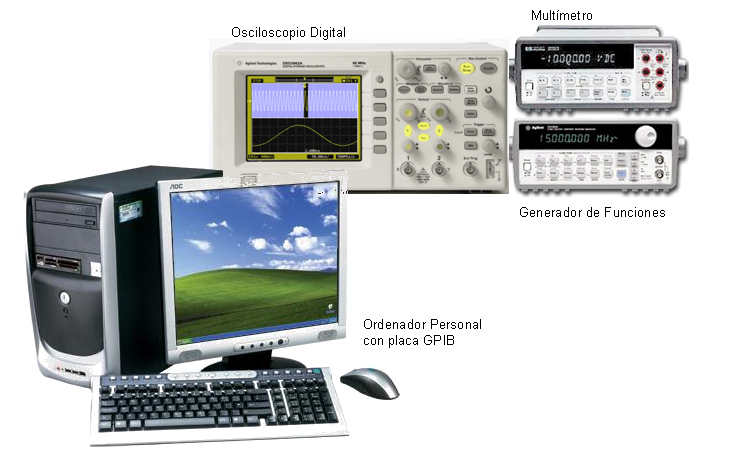
\includegraphics[width=0.9\textwidth]{capturas/entorno}
 \caption{Puesto de Trabajo}
 \label{fig:entorno}
\end{figure}

\subsection{Entorno de trabajo}

Iniciamos LabView y exploramos las diferentes utilidades y paletas de herramientas, controles y funciones. Descubrimos que los bloques de color amarillo que aparecen en algunas subpaletas de funciones se tratan:

\begin{itemize}
 \item Elementos operacionales fundamentales deLABVIEW que no tienen panel frontal ni diagrama de bloques.
 \item SubVi's generados por el usuario.
\end{itemize}

\subsection{Generador Sinusiodal}

Siguiendo los pasos indicados en la Gu\'ia de pr\'acticas de laboratorio, construimos el generador de se\~nal sinusoidal y comprobamos su correcto funcionamiento. Ver figura \ref{fig:gen-sin}

\begin{figure}[H]
 \centering
 \subfloat[Panel Frontal]{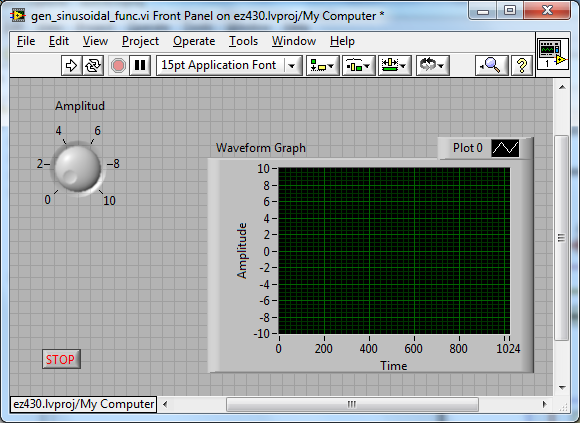
\includegraphics[width=0.4\textwidth]{capturas/genSinFront}}
 \vspace{0.5cm}
 \subfloat[Diagrama de Bloques]{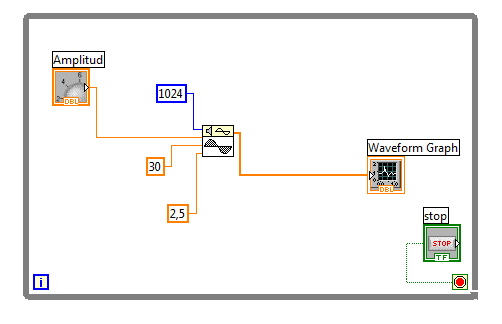
\includegraphics[width=0.4\textwidth]{capturas/genSinBloq}}
 \vspace{0.3cm}
 \caption{Generador Senoidal}
 \label{gen-sin}
\end{figure}


\subsection{Orden de ejecuci\'on}

Despu\'es de analizar el diagrama de la Figura \ref{fig:ej4}, podemos afirmar que el orden de ejecuci\'on del programa ser\'a el siguiente, siguiendo la nomenclatura que se ha dado a los bloques en la figura:

En primer lugar se ejecutar\'a el A, que recibe las entradas del programa. Acto seguido, el bloque B y luego el C. Llegados a este punto, el D precisar\'a de una entrada que es generada por F, por lo que el bloque F se ejecutar\'a tras el B. Luego le seguir\'an en D y el E.

En resumen, el orden de ejecuci\'on ser\'a el siguiente: A - B - C - F - D - E

\begin{figure}[H]
 \centering
 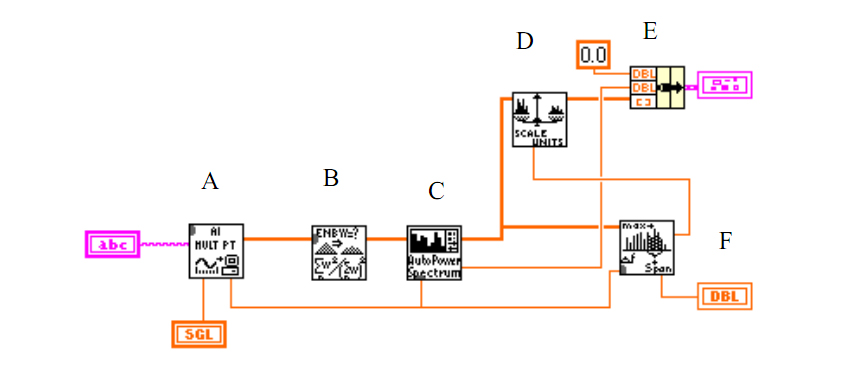
\includegraphics[width=0.7\textwidth]{capturas/ejercicio4}
 \caption{Programa en LatView}
 \label{fig:ej4}
\end{figure}

\subsection{Dise\~no de un generador virtual de se\~nales}

Se\~nales: Sinusoidal, cuadrada y triangular.
Amplitud: Variable entre 0 y 10 Voltios.
Frecuencia: Variable entre 0 Hz y 10 kHz.


Adem\'as hemos incorporado una funcionalidad que permite desplazar la se\~nal en el eje temporal con un control circular que vaya de 0 a 360 y que controle la fase (en grados). En la Figura \ref{fig:front-panels} se puede ver el panel frontal del generador para cada uno de los tres tipos de se\~nal.

\begin{figure}[H]
 \centering
 \subfloat[Se\~nal sinusoidal]{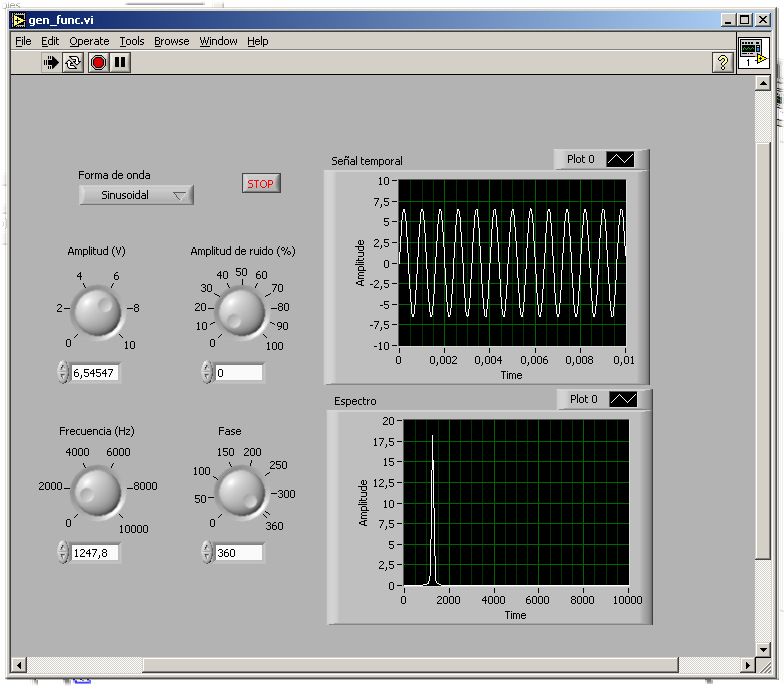
\includegraphics[width=0.4\textwidth]{capturas/frontSinusNoRuido}}
 \hspace{.5cm}
 \subfloat[Se\~nal cuadrada]{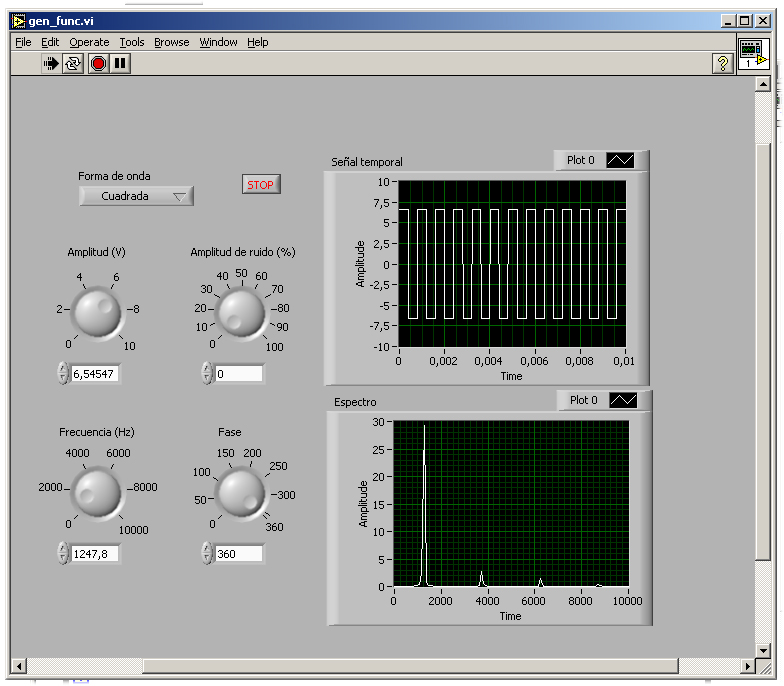
\includegraphics[width=0.4\textwidth]{capturas/frontCuadradaNoRuido}}
 \hspace{.5cm}
 \subfloat[Se\~nal triangular]{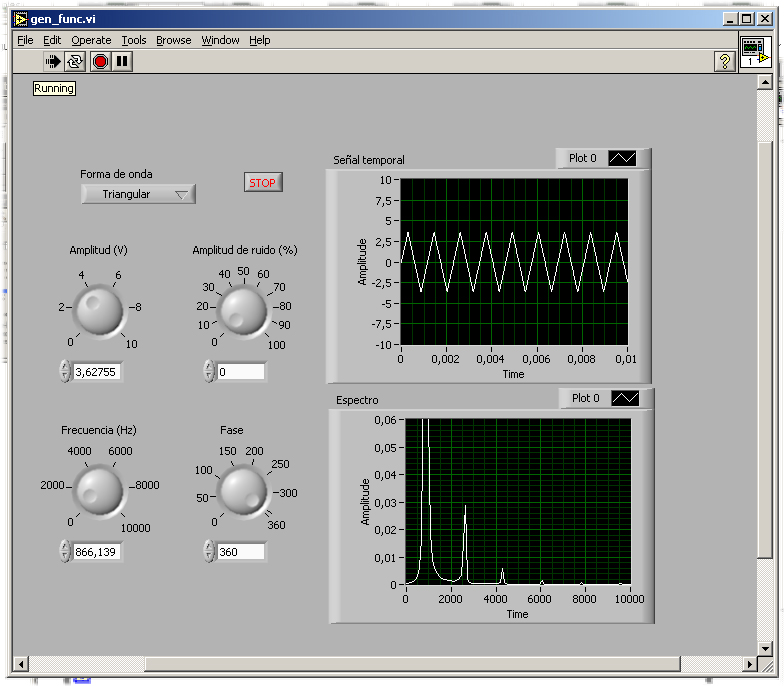
\includegraphics[width=0.8\textwidth]{capturas/frontTriNoRuido}}
 \hspace{.5cm}
 \caption{Panel Frontal del Generador}
 \label{fig:front-panels}
\end{figure}


El diagrama de bloques implementado Se puede ver en la Figura \ref{fig:bloques}. Se muestran las vistas para cada uno de los diferentes casos de la estructura \emph{case}.

\begin{figure}[H]
 \centering
 \subfloat[Se\~nal sinusoidal]{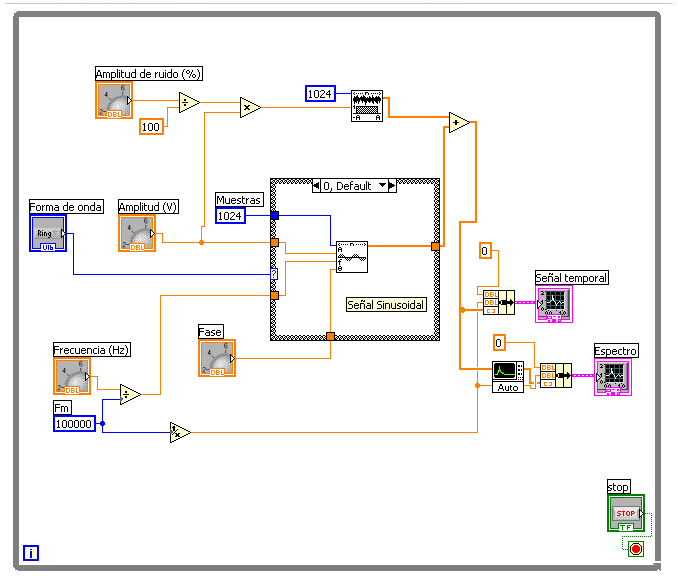
\includegraphics[width=0.4\textwidth]{capturas/bloquesSinus}}
 \hspace{.5cm}
 \subfloat[Se\~nal cuadrada]{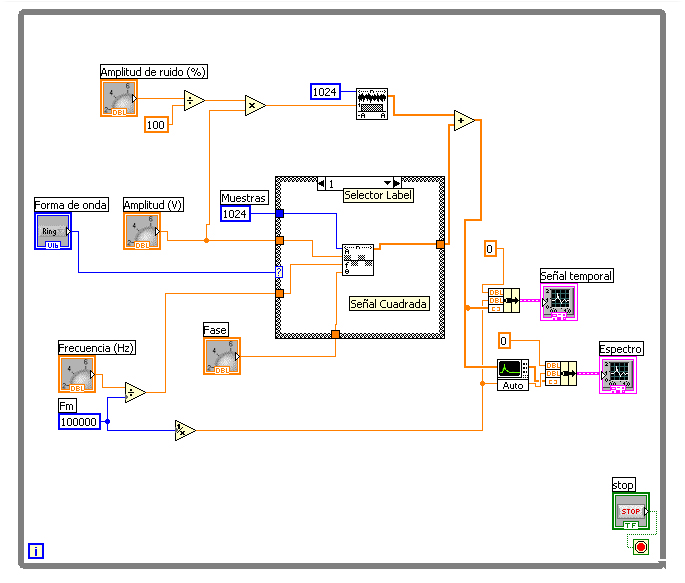
\includegraphics[width=0.4\textwidth]{capturas/bloquesCuadrada}}
 \hspace{.5cm}
 \subfloat[Se\~nal triangular]{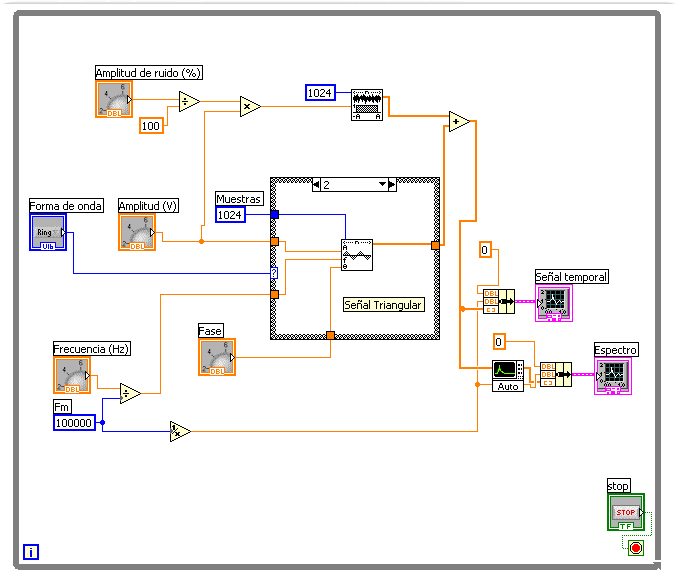
\includegraphics[width=0.8\textwidth]{capturas/bloquesTri}}
 \hspace{.5cm}
 \caption{Vistas del Diagrama de Bloques}
 \label{fig:bloques}
\end{figure}


\section{Trabajo opcional}

Como se puede ver, las capturas de pantalla que se incluyen en las figuras \ref{fig:front-panels} y \ref{fig:bloques} incluyen la mejora que se pide en el trabajo opcional propuesto.

\subsection{Visualizaci\'on del espectro}

Como podemos observar en el detalle de la figura \ref{fig:detalle-espectro}, hemos utilizado una funci\'on sencilla de LabView que proporciona el espectro de una se\~nal mediante las muestras de la misma y su periodo de muestreo. El resultado lo agrupamos en un string y es interpretado por un display de se\~nal. En la figura \ref{fig:front-panels} pueden verse los resultados en el terminal inferior del panel frontal.

\begin{figure}[H]
 \centering
 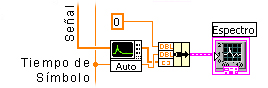
\includegraphics[width=0.5\textwidth]{capturas/detalle-espectro}
 \caption{Detalle del algoritmo para visualizar el espectro}
 \label{fig:detalle-espectro}
\end{figure}


\subsection{Generador de ruido regulable}

Se ha incorporado un algoritmo sencillo (ver figura \ref{fig:detalle-ruido})que permite agregar una componente ruido uniforme con amplitud regulable entre el 0 y el 100\% de la amplitud de la se\~nal original. En la figura \ref{fig:front-panels} puede verse el control circular superior derecho, con la etiqueta \emph{Amplitud de ruido (\%)} que es con el que regulamos el porcentaje de ruido respecto de la amplitud de se\~nal que queremos agregar. 

\begin{figure}[H]
 \centering
 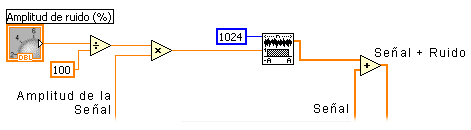
\includegraphics[width=0.5\textwidth]{capturas/detalle-ruido}
 \caption{Detalle del algoritmo para agregar ruido}
 \label{fig:detalle-ruido}
\end{figure}


A continuaci\'on se a\~naden algunas capturas de pantalla para ver el resultado de cada tipo de se\~nal que podemos generar afectada por nuestro ruido aditivo.

\begin{figure}[H]
 \centering
 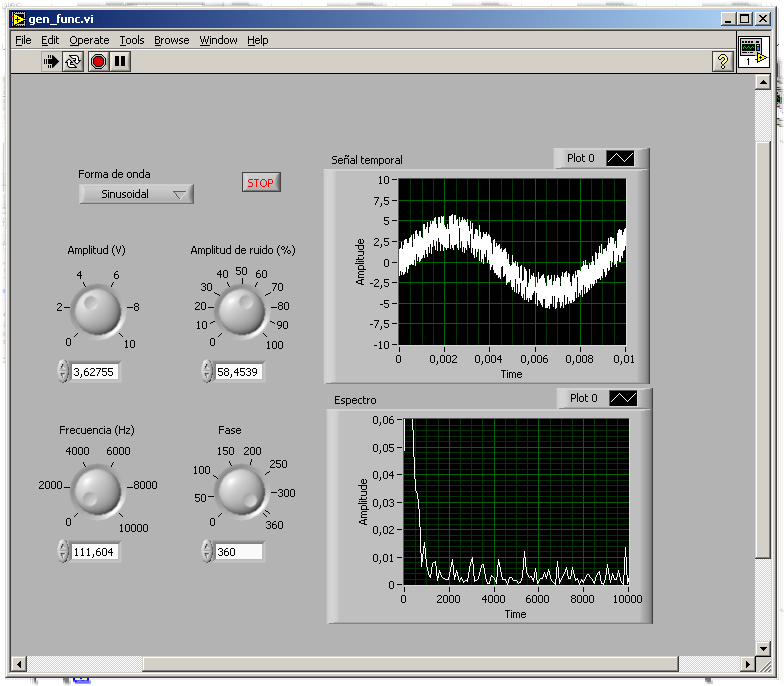
\includegraphics[width=0.5\textwidth]{capturas/frontSinusSiRuido}
 \caption{Se\~nal sinusoidal + ruido}
 \label{fig:front-sinus-noise}
\end{figure}


\begin{figure}[H]
 \centering
 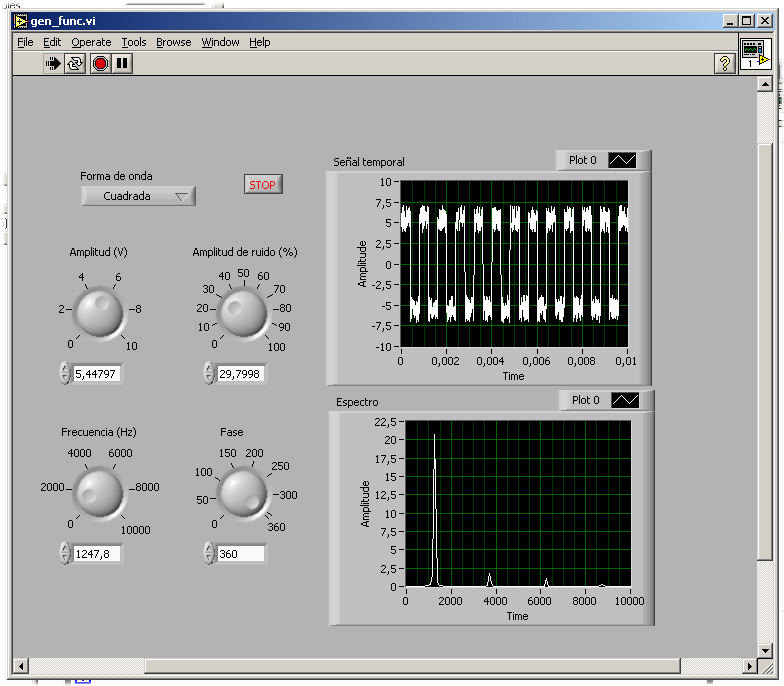
\includegraphics[width=0.5\textwidth]{capturas/frontCuadradaSiRuido}
 \caption{Se\~nal cuadrada + ruido}
 \label{fig:front-square-noise}
\end{figure}


\begin{figure}[H]
 \centering
 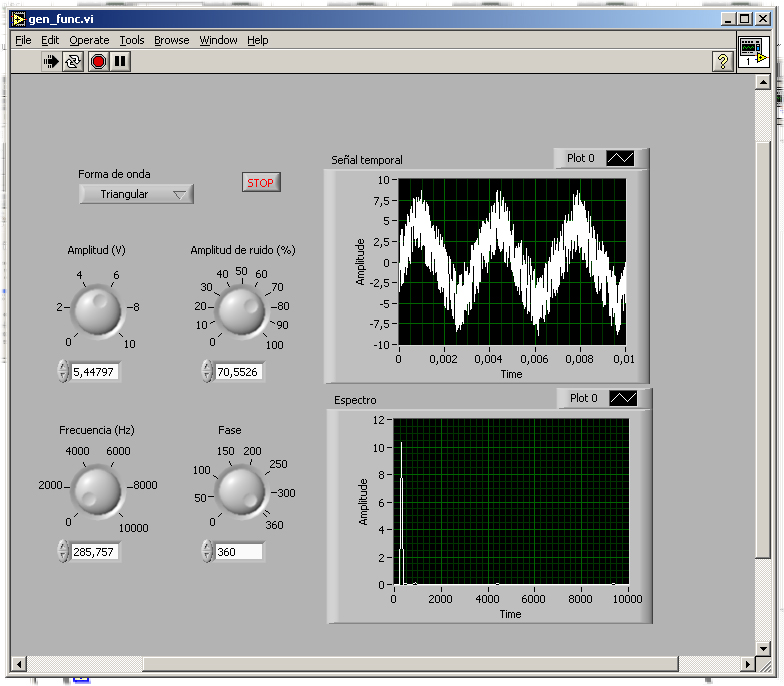
\includegraphics[width=0.5\textwidth]{capturas/frontTriSiRuido}
 \caption{Se\~nal triangular + ruido}
 \label{fig:front-tri-noise}
\end{figure}


\end{document}